%%%%%%%%%%%%%%%%%%%%%%%%%%%%%%%%%%%%%%%%%%%%%%%%%%%%%%%%%%%%%%%%%%%%
%% I, the copyright holder of this work, release this work into the
%% public domain. This applies worldwide. In some countries this may
%% not be legally possible; if so: I grant anyone the right to use
%% this work for any purpose, without any conditions, unless such
%% conditions are required by law.
%%%%%%%%%%%%%%%%%%%%%%%%%%%%%%%%%%%%%%%%%%%%%%%%%%%%%%%%%%%%%%%%%%%%

\documentclass{beamer}
\usetheme[faculty=law,logoPath=./,logo=fudan_logo_vector.eps]{fibeamer}
\usepackage[utf8]{inputenc}
\usepackage{fontspec}
\setsansfont[Scale=MatchLowercase,Mapping=tex-text]{Calibri}
\setmonofont[Scale=MatchLowercase]{Courier New}  
\usepackage[
  % main=english, %% By using `czech` or `slovak` as the main locale
                %% instead of `english`, you can typeset the
                %% presentation in either Czech or Slovak,
                %% respectively.
    czech, 
    slovak,english, %% The additional keys allow foreign texts to be
]{babel}        %% typeset as follows:
%%
%%   \begin{otherlanguage}{czech}   ... \end{otherlanguage}
%%   \begin{otherlanguage}{slovak}  ... \end{otherlanguage}
%%
%% These macros specify information about the presentation
\title{Anisotropic in-plane thermal conductivity observed in multilayer silicene} %% that will be typeset on the
%% \subtitle{} %% title page.
\author{Yang Zhou}
%% These additional packages are used within the document:
\usepackage{ragged2e}  % `\justifying` text
\usepackage{booktabs}  % Tables
\usepackage{tabularx}
\usepackage{tikz}      % Diagrams
\usetikzlibrary{calc, shapes, backgrounds}
\usepackage{amsmath, amssymb}
\usepackage{url}       % `\url`s
\usepackage{listings}  % Code listings
\usepackage{color}

\frenchspacing
\begin{document}
\uselanguage{english}
\frame{
\maketitle \\
{\color{white} \today}
}


\begin{frame}<beamer>
  \frametitle{Outline} %%\thesection
  \tableofcontents
\end{frame}


\section{Structures}
\begin{frame}{Structures}
  \framesubtitle{Multilayer Silicenes}%
  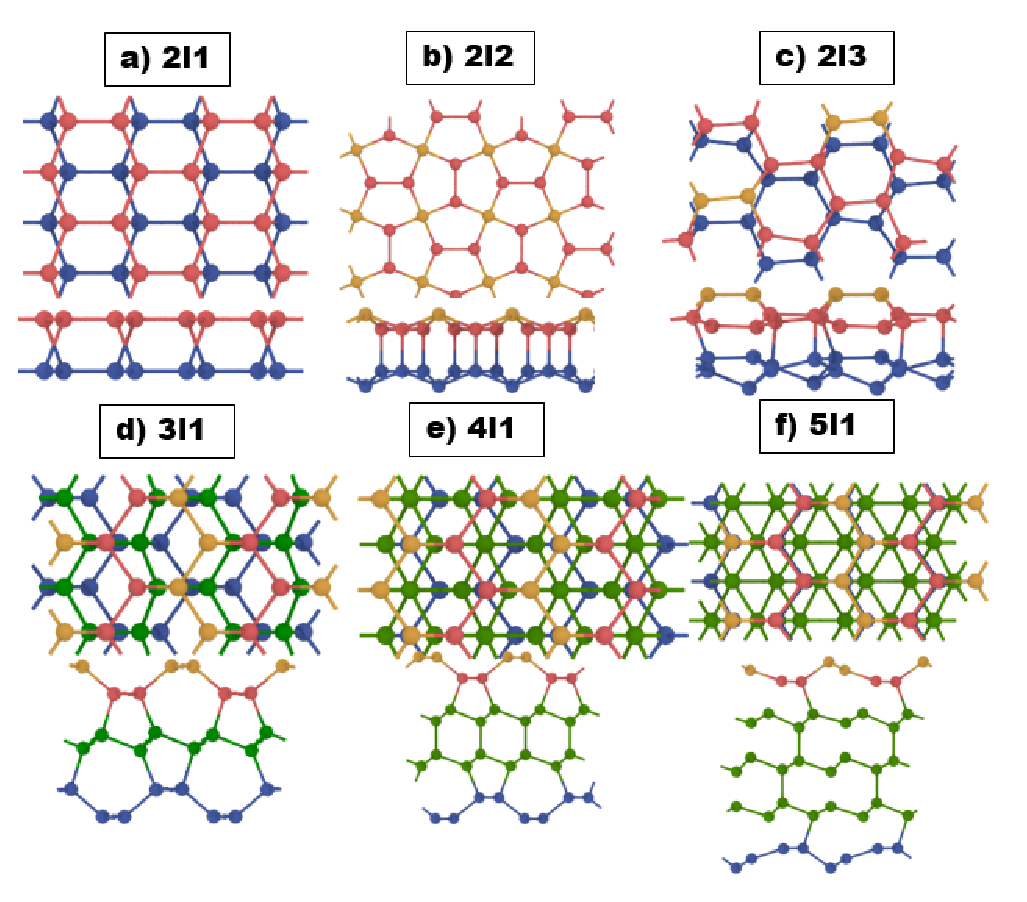
\includegraphics[width=\textwidth]{images/structures}
\end{frame}

\begin{frame}{Structure Characteristic}
  \framesubtitle{Symmetry,Energy and Surface}%
  \begin{table}[!b]
    \tiny
    {\carlitoTLF % Use monospaced lining figures
      \begin{tabular}{cccccccc}
        \textbf{Name}
             & \textbf{Minimal period}
             & \textbf{Symmetry}
             & \textbf{$\mathbf{E_c}$ in Guo}
             & \textbf{$\mathbf{E_c}$ in MD}
             & \textbf{Buckling Feature}                                                                    \\
        \toprule
        2l1  & $1 \times 1$                   & Cmme    & 5.000 & 4.145 & Smooth                            \\
        2l2  & $\sqrt{2}\times\sqrt{2}$       & C12/m1  & 4.991 & 4.204 & Large buckling and symmetric      \\
        2l3  & $2 \times 2$                   & C12/m1  & 5.063 & 4.257 & Large buckling and tilt symmetric \\
        2lh  & $2 \times 2$                   & P1      & 5.073 & 4.216 & Large buckling                    \\
        2lr3 & $\sqrt{3}\times\sqrt{3}$       & P1      & -     & 4.225 & Small buckling and symmetric      \\
        3l1  & $2 \times 1$                   & P121/m1 & 5.138 & 4.337 & -                                 \\
        3l2  & $2 \times 1$                   & P1      & 5.135 & 4.298 & -                                 \\
        4l1  & $2 \times 1$                   & P1      & 5.225 & 4.368 & -                                 \\
        2l2  & $\sqrt{2}\times\sqrt{2}$       & C12/m1  & 4.991 & 4.204 & Large buckling and symmetric      \\
        2l3  & $2 \times 2$                   & C12/m1  & 5.063 & 4.257 & Large buckling and tilt symmetric \\
        2lh  & $2 \times 2$                   & P1      & 5.073 & 4.216 & Large buckling                    \\
        2lr3 & $\sqrt{3}\times\sqrt{3}$       & P1      & -     & 4.225 & Small buckling and symmetric      \\
        3l1  & $2 \times 1$                   & P121/m1 & 5.138 & 4.337 & -                                 \\
        3l2  & $2 \times 1$                   & P1      & 5.135 & 4.298 & -                                 \\
        4l1  & $2 \times 1$                   & P1      & 5.225 & 4.368 & -                                 \\
        \bottomrule
      \end{tabular}
    }

    \caption{
      Symmetry of the structures, binding energy $E_c(eV/Si)$ and structure features}
  \end{table}

\end{frame}

\section{Effect of Buckling $\&$ Layers on TC}
\begin{frame}{Effect of Buckling on TC}
  \framesubtitle{$\kappa = \kappa_\infty (1-e^{-\frac{L}{L_c}})$}%

  \begin{columns}[onlytextwidth]
    \tiny
    \column{.5\textwidth}
    The letter z/a in the legend mean the transport direction is zigzag/armchair.\\
    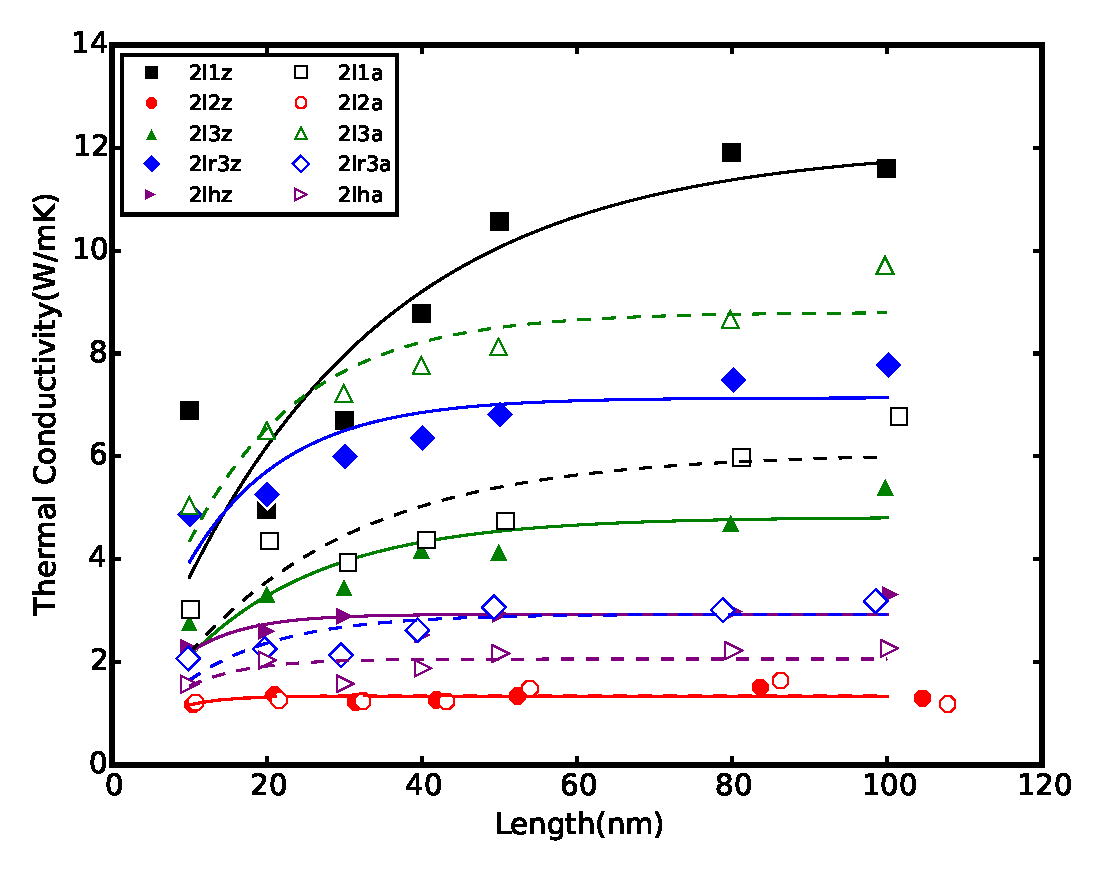
\includegraphics[width=\textwidth]{images/2l_length}

    \column{.5\textwidth}
    TC along zigzag are larger than armchair while anisotropy decrese when layer increases.\\
    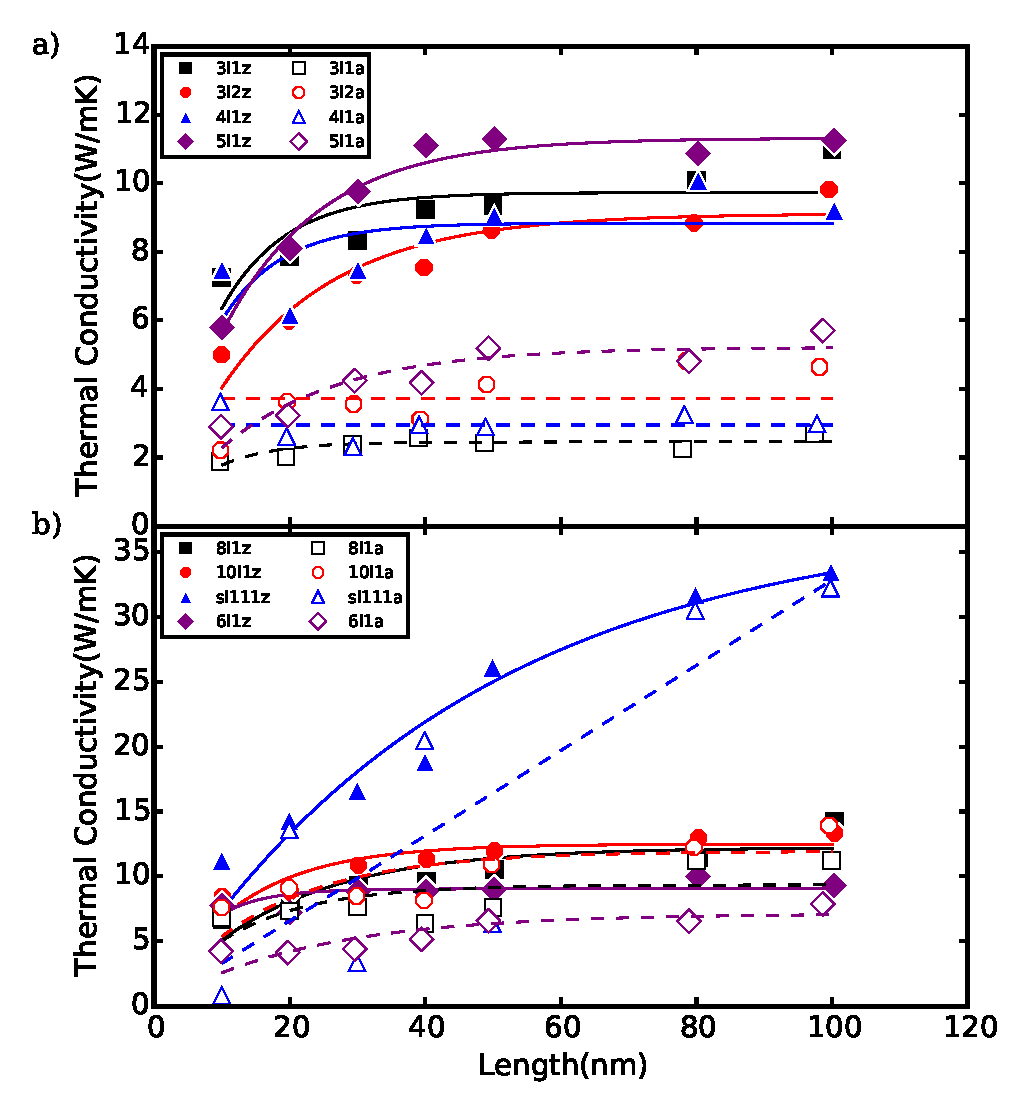
\includegraphics[width=\textwidth]{images/vl_length}

  \end{columns}

\end{frame}



\section{Anisotropy of Thermal Conductivity}
\begin{frame}{Anisotropy of Thermal Conductivity}
  \framesubtitle{Diffusive TC of varible structures}%
  $ \chi=|\kappa_{z,\infty}-\kappa_{a,\infty} |/max⁡(\kappa_{z,\infty}-\kappa_{a,\infty} ) \times 100 \%$
  \begin{table}[!b]
    \tiny
    {\carlitoTLF % Use monospaced lining figures
      \begin{tabular}{cccccccccccc}
              & \textbf{$\mathbf{\kappa_{z,\infty}}$}
              & \textbf{$\mathbf{\kappa_{a,\infty}}$}
              & \textbf{$\mathbf{\chi}$}
              & $Cv_{z}$
              & $Cv_{a}$
              &
              & \textbf{$\mathbf{\kappa_{z,\infty}}$}
              & \textbf{$\mathbf{\kappa_{a,\infty}}$}
              & \textbf{$\mathbf{\chi}$}
              & $Cv_{z}$
              & $Cv_{a}$                                                                                                                \\
        \toprule
        2l1   & 11.6                                  & 6.5  & 43.9\% & 165.8 & 166.7 & 2l2      & 1.5  & 1.2  & 20.0\% & 38.44 & 38.44 \\
        2l3   & 5.0                                   & 9.7  & 48.5\% & 23.38 & 23.38 & 2lr3     & 8.2  & 3.5  & 57.3\% & 10.15 & 10.15 \\
        2lh   & 2.0                                   & 2.5  & 20.0\% & 22.42 & 22.42 & 3l1      & 11.5 & 2.9  & 74.8\% & 52.22 & 52.46 \\
        3l2   & 10.2                                  & 5.2  & 49.0\% & 55.56 & 55.84 & 4l1      & 10.2 & 3.4  & 66.7\% & 37.71 & 37.89 \\
        5l1   & 11.7                                  & 5.7  & 51.3\% & 29.17 & 29.32 & 6l1      & 10.3 & 7.8  & 24.3\% & 23.73 & 23.86 \\
        8l1   & 13.2                                  & 14.9 & 11.4\% & 17.26 & 17.36 & 10l1     & 13.3 & 13.5 & 1.5\%  & -     & -     \\
        Si111 & 33.6                                  & 34.7 & 3.2\%  & -     & -     & Silicene & 11.4 & 11.6 & 1.7\%  & 606.4 & 613.4 \\
        \bottomrule
      \end{tabular}
    }
    \caption{
      The thermal conductivity and anisotropic ratio of different multi-layer silicene.}
  \end{table}

\end{frame}

\section{Phonon Dispersion}
\begin{frame}{Phonon Dispersion}
  \begin{figure}[b]
    \begin{columns}[onlytextwidth]
      \column{.5\textwidth}
      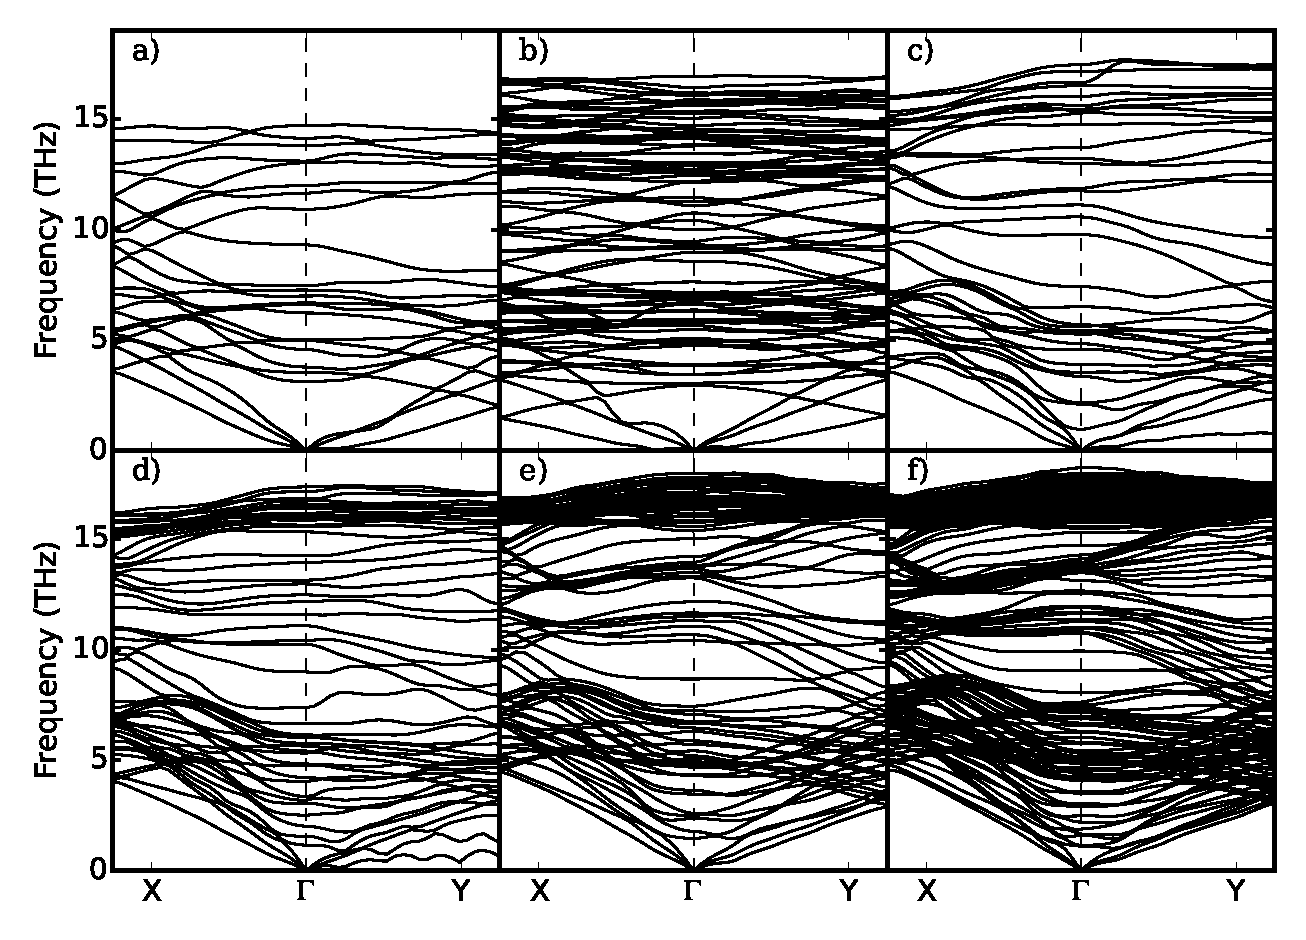
\includegraphics[width=0.8\textwidth]{images/bands}
      \caption{\label{fig:bands} $\Gamma(0.0, 0.0, 0.0)$, $X(0.5, 0.0, 0.0)$,  $Y(0.0, 0.5, 0.0)$}
      \column{.5\textwidth}
      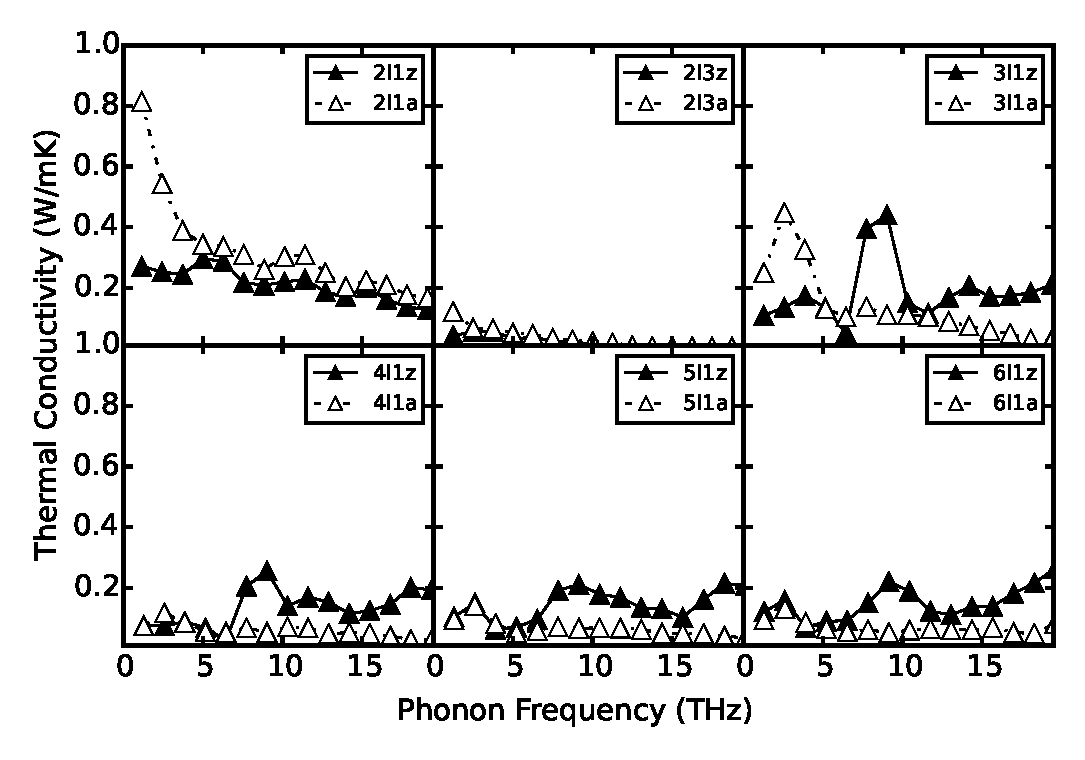
\includegraphics[width=\textwidth]{images/tc_freq}
      \caption{\label{fig:freq} The contribution of thermal conductivity from different frequency }
    \end{columns}
  \end{figure}
\end{frame}

\section{Thermal Condcutivity Tensor}
\begin{frame}{Thermal Condcutivity Tensor}
  \framesubtitle{Heat Capacity $\&$ Group Velocity}%
  $\kappa^{\alpha\beta} = \sum_{k \sigma}{c_{k \sigma}v^{\alpha}_{k \sigma}v^{\beta}_{k \sigma}\tau_{k \sigma}}$

  \begin{columns}[onlytextwidth]
    \column{.8\textwidth}
    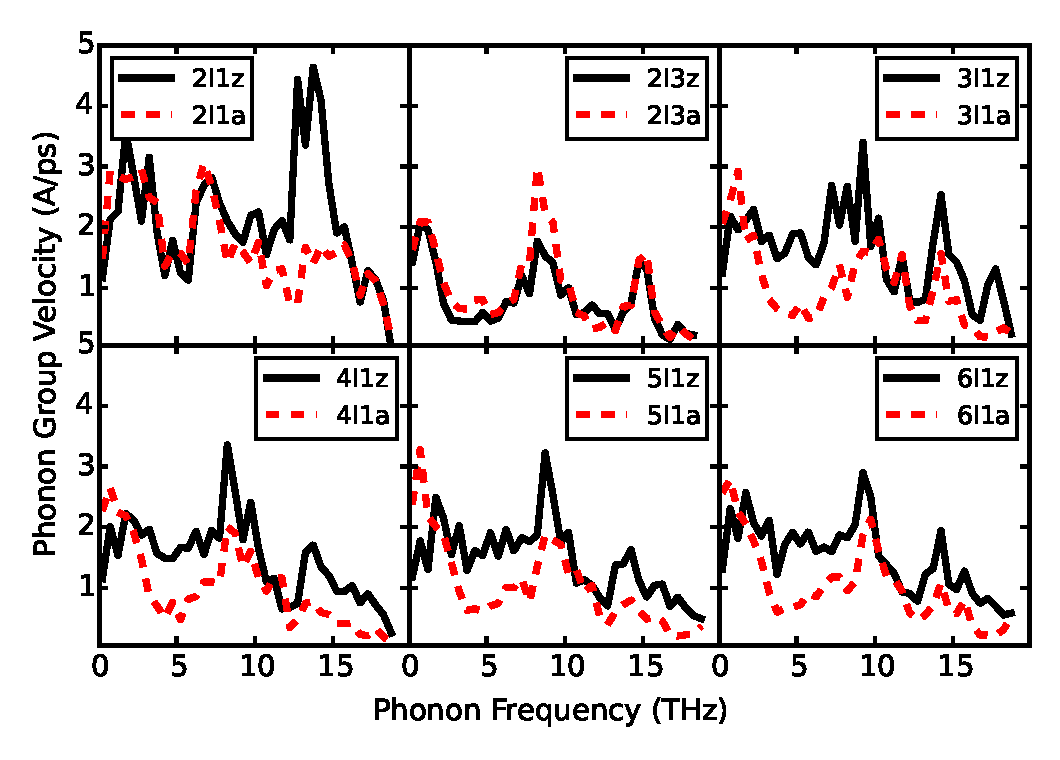
\includegraphics[width=\textwidth]{images/gv}
  \end{columns}
\end{frame}

\section{Phonon Localization}
\begin{frame}{Phonon Localization}
  \framesubtitle{Participation Ratio $\&$ Transmission}%
  \begin{columns}[onlytextwidth]
    \column{.5\textwidth}
    \includegraphics[width=\textwidth]{images/pr_direction}
    \column{.5\textwidth}
    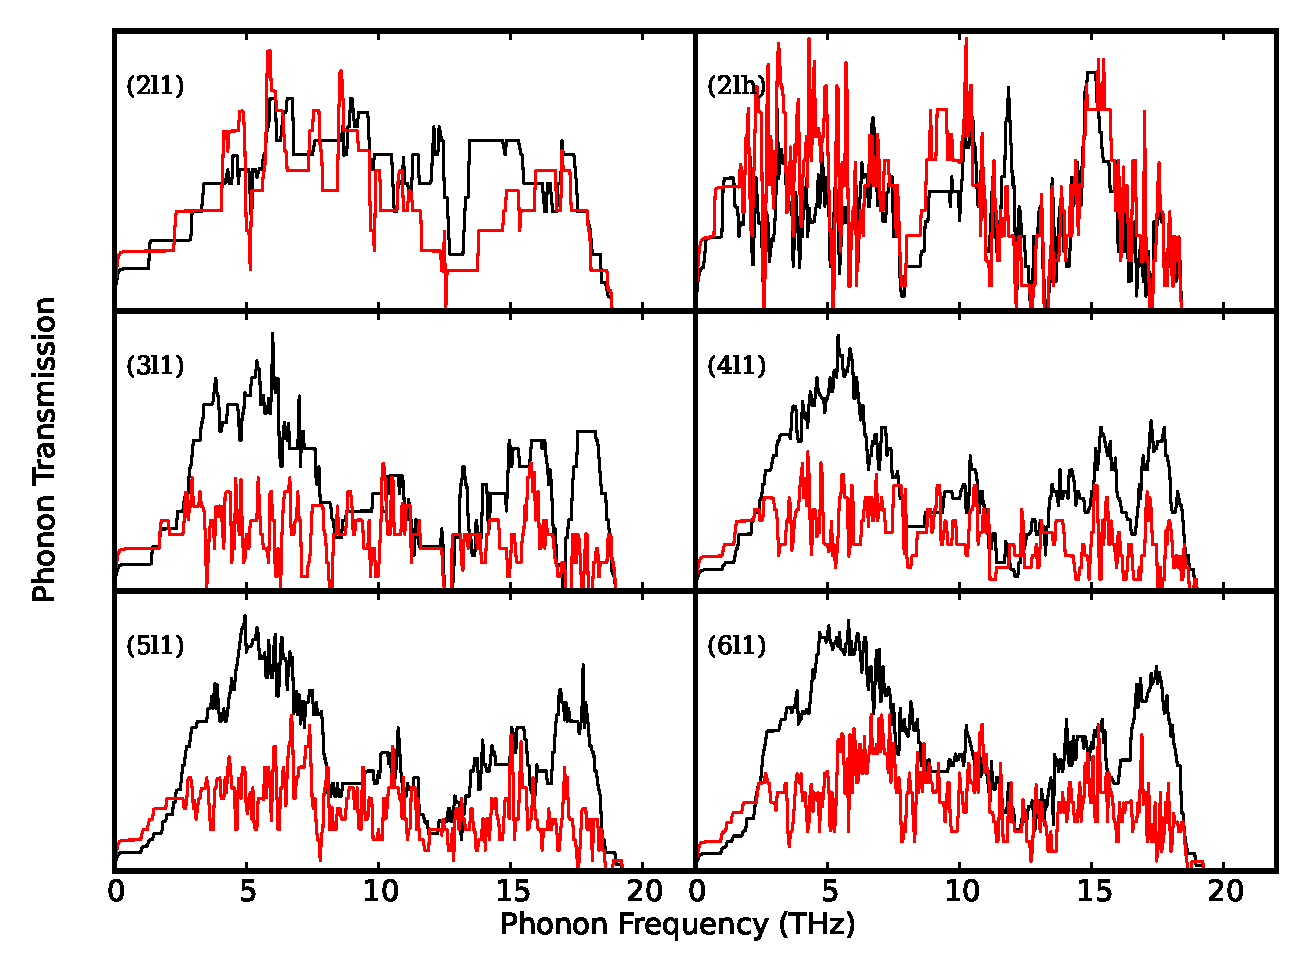
\includegraphics[width=\textwidth]{images/transmission}
  \end{columns}
\end{frame}

\section{Phonon Scattering}
\begin{frame}{Phonon Scattering}
  \framesubtitle{Lifetime $\&$ Gruneisen Parameter}%
  \begin{columns}[onlytextwidth]
    \column{.5\textwidth}
    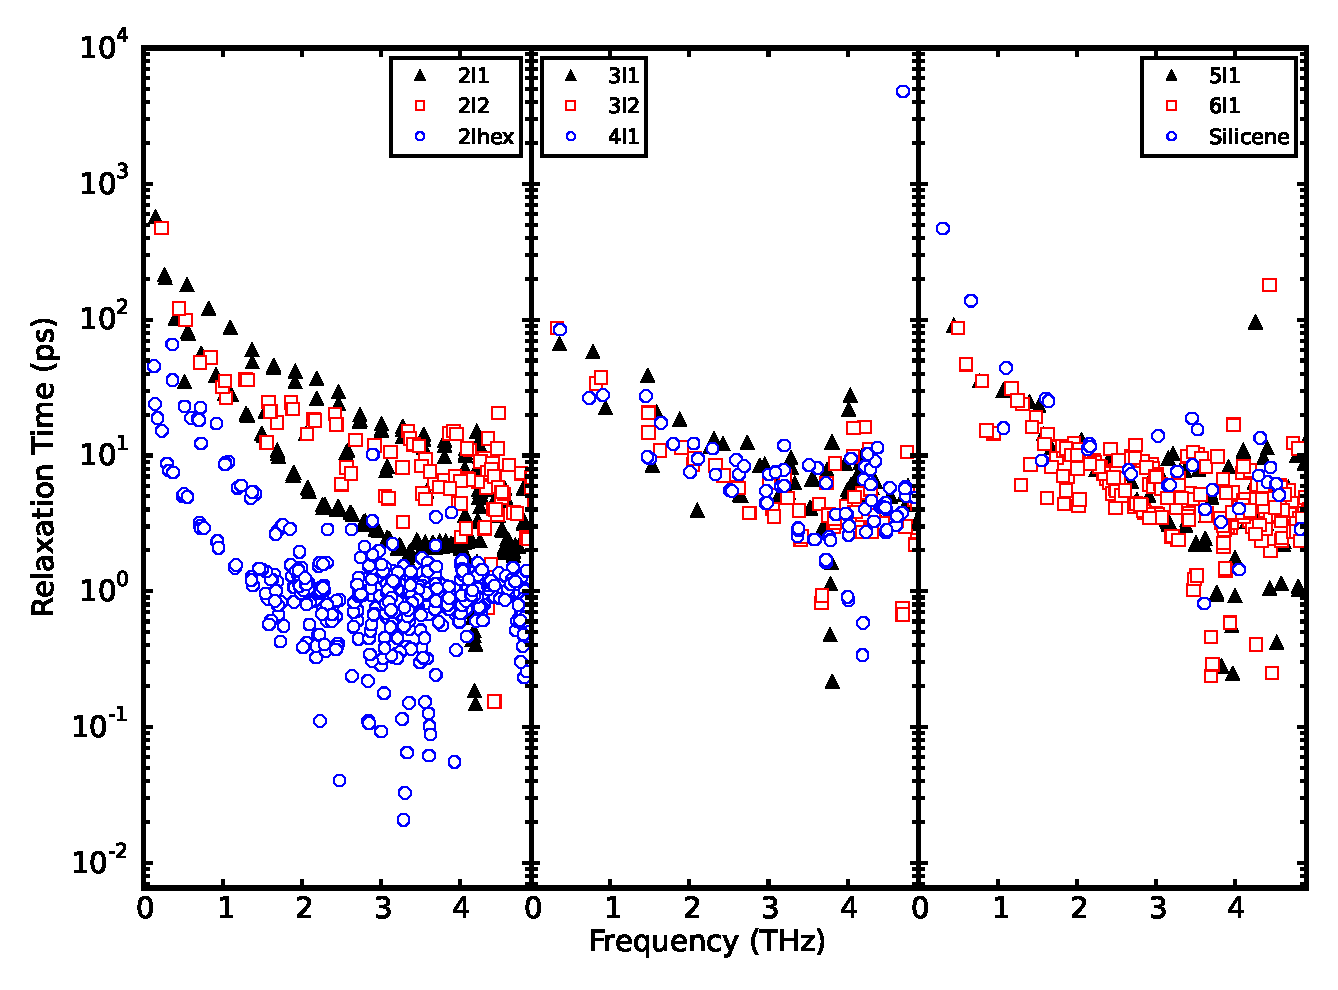
\includegraphics[width=\textwidth]{images/tau}
    \column{.5\textwidth}
    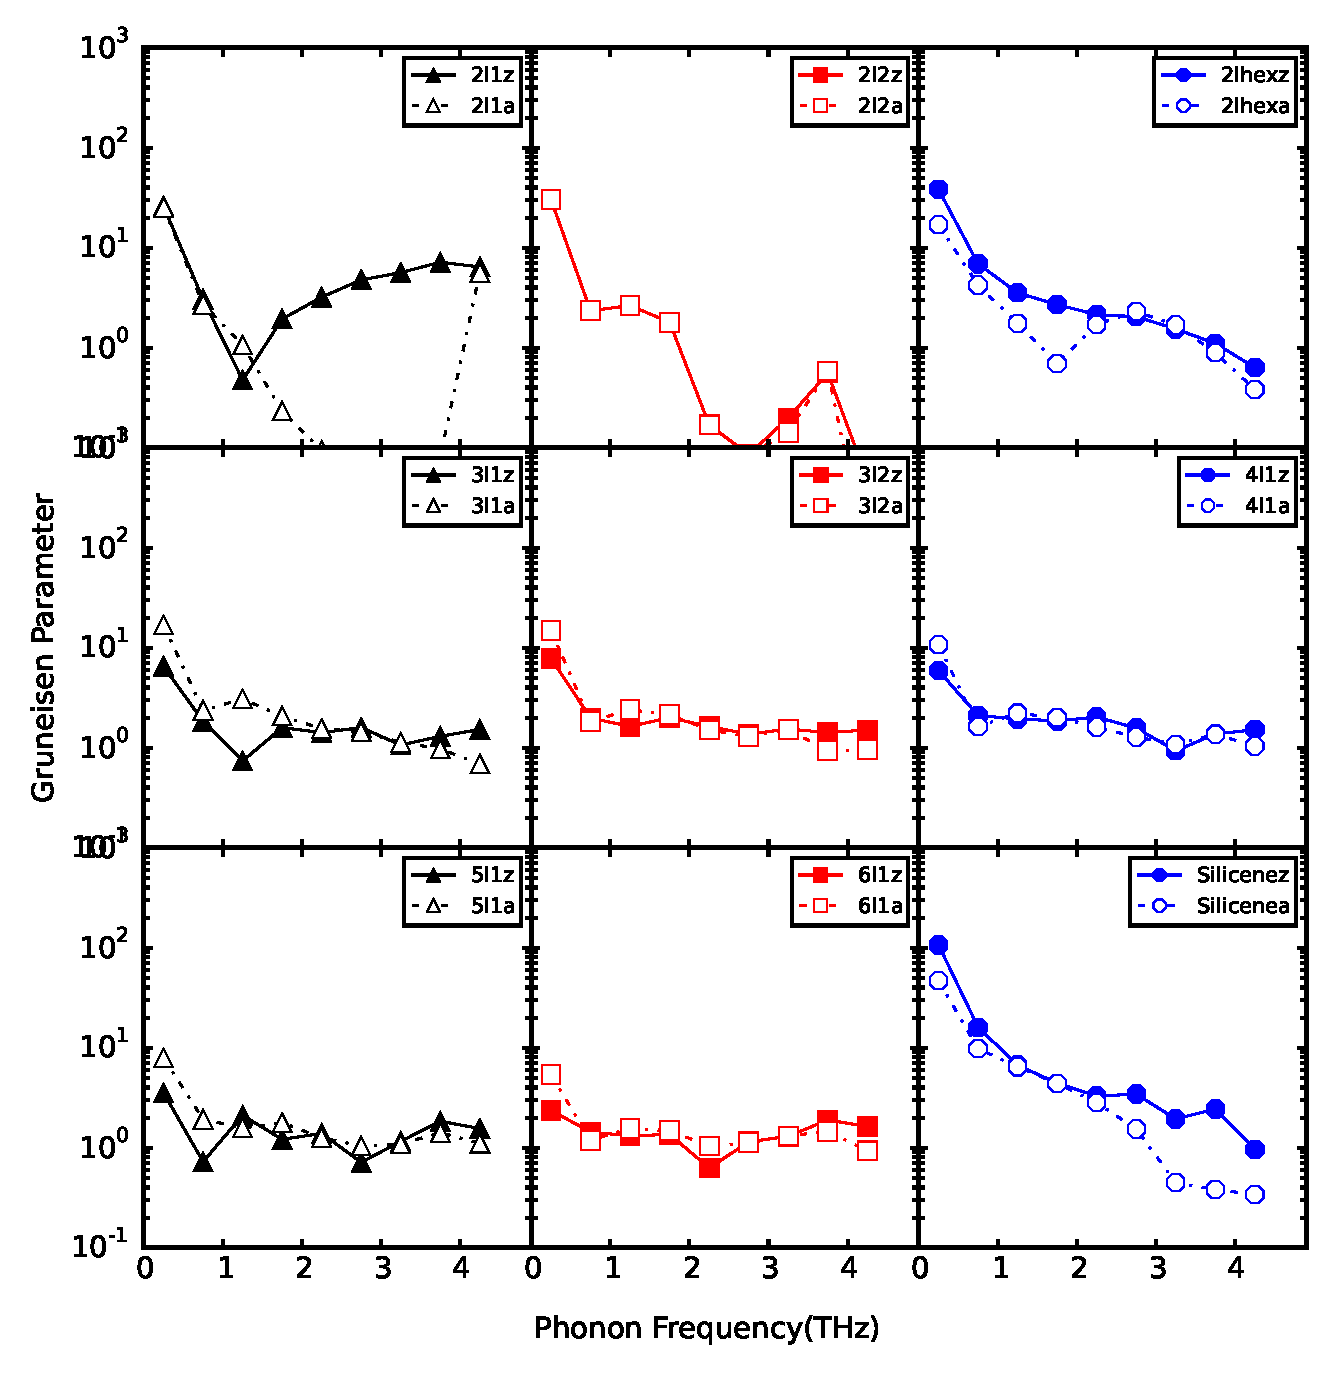
\includegraphics[width=\textwidth]{images/gruneisen}
  \end{columns}
\end{frame}

\section{Conclusion}
\begin{frame}[label=lists]{Conclusion}

  \begin{enumerate}
    \item layer < 6L
          \begin{itemize}
            \item Large anisotropy(>20\%).
          \end{itemize}
          \begin{itemize}
            \item Reason: Group velosity differrence caused by reconstruction.
          \end{itemize}
    \item layer = 2L
          \begin{itemize}
            \item Most difference due to reconstruction.
          \end{itemize}
          \begin{itemize}
            \item More layer will reduce reconstruction so the anisotropy.
          \end{itemize}
    \item layer < 6L
          \begin{itemize}
            \item TC as low as 1.2 W/mK
          \end{itemize}
          \begin{itemize}
            \item Anisotropy as high as 75\%
          \end{itemize}

          \begin{itemize}
            \item Potential in thermoelectric application
          \end{itemize}
  \end{enumerate}
  \bigskip
  \justifying

\end{frame}


\begin{frame}[label=bibliography]{Bibliography}
  \framesubtitle{\TeX, \LaTeX, and Beamer}
  \begin{thebibliography}{9}
    \bibitem{knuth84}
    Donald~E.~Knuth.
    \emph{The \TeX book}.
    Addison-Wesley, 1984.
    \bibitem{lamport94}
    Leslie~Lamport.
    \emph{\LaTeX : A Document Preparation System}.
    Addison-Wesley, 1986.
    \bibitem{MG94}
    M.~Goossens, F.~Mittelbach, and A.~Samarin.
    \emph{The \LaTeX\ Companion}.
    Addison-Wesley, 1994.
    \bibitem{tantau04}
    Till~Tantau.
    \emph{User's Guide to the Beamer Class Version 3.01}.
    Available at \url{http://latex-beamer.sourceforge.net}.
    \bibitem{MS05}
    A.~Mertz and W.~Slough.
    Edited by B.~Beeton and K.~Berry.
    \emph{Beamer by example} In TUGboat,
    Vol. 26, No. 1., pp. 68-73.
  \end{thebibliography}
\end{frame}


\end{document}
